\documentclass[tikz,border=8pt]{standalone}
\usepackage{amsmath}
\usetikzlibrary{arrows.meta}
\definecolor{ink}{HTML}{21352F}
\definecolor{teal}{HTML}{087F7B}
\definecolor{blue}{HTML}{4B77A8}
\definecolor{gold}{HTML}{C58B2A}
\definecolor{rose}{HTML}{B65A62}
\begin{document}
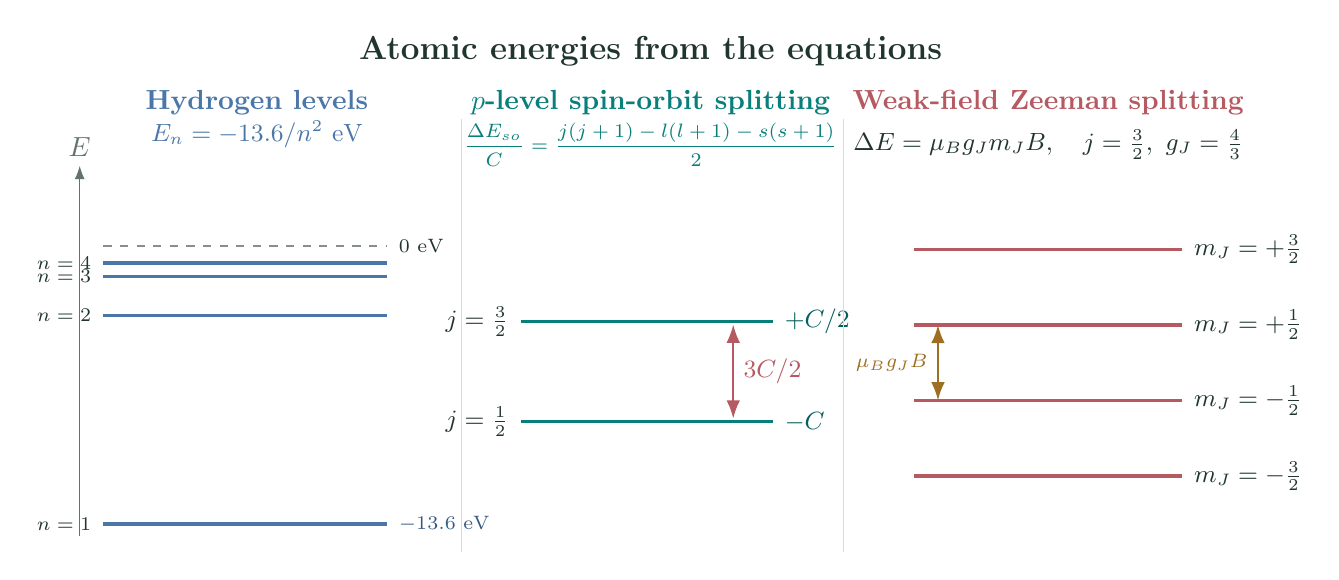
\begin{tikzpicture}[font=\sffamily,text=ink,>=Latex]
  \node[font=\bfseries\large] at (0,6.0)
    {Atomic energies from the equations};

  \node[font=\bfseries,text=blue] at (-5.0,5.35)
    {Hydrogen levels};
  \node[font=\small,text=blue] at (-5.0,4.95)
    {$E_n=-13.6/n^2$ eV};
  \draw[->,ink!70] (-7.25,-.15)--(-7.25,4.55) node[above] {$E$};
  \foreach \n in {1,...,4}{
    \pgfmathsetmacro{\en}{-13.6/(\n*\n)}
    \pgfmathsetmacro{\yy}{0.26*(13.6+\en)}
    \draw[blue,very thick] (-6.95,\yy)--(-3.35,\yy);
    \node[left,font=\scriptsize] at (-6.98,\yy)
      {$n=\n$};
  }
  \node[right,font=\scriptsize,text=blue!75!black]
    at (-3.32,0) {$-13.6$ eV};
  \pgfmathsetmacro{\yion}{0.26*13.6}
  \draw[ink!55,dashed,thick] (-6.95,\yion)--(-3.35,\yion);
  \node[right,font=\scriptsize] at (-3.32,\yion) {$0$ eV};

  \draw[ink!18] (-2.4,-.35)--(-2.4,5.15);
  \node[font=\bfseries,text=teal] at (0,5.35)
    {$p$-level spin-orbit splitting};
  \node[font=\scriptsize,text=teal,align=center] at (0,4.82)
    {$\displaystyle\frac{\Delta E_{so}}C=
      \frac{j(j+1)-l(l+1)-s(s+1)}2$};
  \def\base{2.15}
  \def\scale{0.85}
  \pgfmathsetmacro{\yhalf}{\base+\scale*(-1)}
  \pgfmathsetmacro{\ythree}{\base+\scale*(0.5)}
  \draw[teal,very thick] (-1.65,\yhalf)--(1.55,\yhalf);
  \draw[teal,very thick] (-1.65,\ythree)--(1.55,\ythree);
  \node[left,font=\small] at (-1.68,\yhalf) {$j=\tfrac12$};
  \node[left,font=\small] at (-1.68,\ythree) {$j=\tfrac32$};
  \node[right,font=\small,text=teal!75!black]
    at (1.58,\yhalf) {$-C$};
  \node[right,font=\small,text=teal!75!black]
    at (1.58,\ythree) {$+C/2$};
  \draw[<->,rose,thick] (1.05,\yhalf+.04)--(1.05,\ythree-.04)
    node[midway,right,font=\small] {$3C/2$};

  \draw[ink!18] (2.45,-.35)--(2.45,5.15);
  \node[font=\bfseries,text=rose] at (5.05,5.35)
    {Weak-field Zeeman splitting};
  \node[font=\small] at (5.05,4.82)
    {$\Delta E=\mu_Bg_Jm_JB,\quad j=\tfrac32,\ g_J=\tfrac43$};
  \foreach \m/\lab in {-1.5/{-\frac32},-0.5/{-\frac12},0.5/{+\frac12},1.5/{+\frac32}}{
    \pgfmathsetmacro{\yy}{2.05+0.72*(4/3)*\m}
    \draw[rose,very thick] (3.35,\yy)--(6.75,\yy);
    \node[right,font=\small] at (6.78,\yy) {$m_J=\lab$};
  }
  \draw[gold!80!black,thick,<->]
    (3.65,{2.05-0.72*(2/3)})--(3.65,{2.05+0.72*(2/3)})
    node[midway,left,font=\scriptsize] {$\mu_Bg_JB$};
\end{tikzpicture}
\end{document}
